\chapter{The tool}

\section{General description}
\label{tool_general_description}
The tool has two components: a \textit{data gatherer} and a \textit{visualization client}.

The data gatherer is a C++ header-only class of which methods have to be called within the main loop of any unidirectional path tracer. It stores to disk data generated --- and usually discarded --- by the path tracer during rendering. For each path shoot by the renderer the tool stores its transported radiance, its camera sample, and the world positions of its bounces. 

Once the rendering is done and the data is collected, the visualization client can be used to explore the gathered information. To allow interactive 3D exploration it also needs a scene description; this is not generated by the gatherer and it has to be provided separately by the user. The scene format used is novel, based on triangle meshes and it shares many similarities with glTF \cite{robinet2014gltf}. This peculiar choice has been done mainly to not do any assumptions on the kind of geometry representation the path tracer uses. In this way even path tracers that use exotic geometries can be analyzed with the tool --- at least until the user is able to convert whatever they are using in triangles.


\section{Data gatherer}

\subsection{The data to gather}
Until now it has been said that the gatherer has to be able to store “the paths with some useful data”, but how does one store a path and what is useful data have not been defined yet. In the beginning, the focus was on just visualizing paths in an interactive scene rendering so that the user could see how paths interact with the scene. To achieve that it was clear the actual geometry of all paths had to be stored. This meant storing for each path a camera sample and all of its bounces.
Several ways of storing path bounces had been considered, such as storing each bounce as a direction and a distance, but the most n\"aive solution has been opted: each bounce is stored as a 3-dimensional point in world space.

This immediately raised some concerns about how much memory would be required to store all these points: let us calculate how many bytes it would take to just store the bounces of all paths needed to produce image \ref{hall_render}. It is 512 pixels wide and 512 pixels tall, it has been rendered with 512 samples per pixel --- spp --- each with a depth of maximum 10 --- this means that each of the 512 paths shoot every pixel bounced in the scene at most 10 times. Storing the points as a triplet of single precision float numbers --- 4 bytes, the C++ built-in \texttt{float} type ---  we would have:
\begin{equation}
	\label{rough_bounce_size_estimation}
	(512 \times 512) pixels \times 512 spp \times 10 bounces \times 3 dimensions \times 4 bytes \approx 15GB
\end{equation}
\begin{figure}
	\centering
	\includegraphics[height=8cm]{chapters/chapter_thetool/hall}
	\caption{\textit{Modern Hall} scene \cite{bitterliscenes} rendered by Yocto/GL \cite{pellacini2019yocto}. It is a 512x512, 512spp image; maximum bounces per path are set to 10.}
	\label{hall_render}
\end{figure}
As said just above, the paths in this case bounce at most 10 times: most paths are terminated way before either when they bounce out of the scene or --- in some path tracers --- they hit a light. This leads to the need of an additional buffer storing the amount of bounces each path has. Put with computer graphics terminology we might say the points positions buffer represents the \textit{geometry} of the paths while this “path lengths” buffer is the \textit{topology}. 
This new buffer needs to contain integers and, considering that the standard C++ \texttt{int} built-in type on x86\_64 machines is 4 bytes long, we would have that the size of the buffer in the context of figure \ref{hall_render} would approximately be:
\begin{equation}
	\label{rough_lenghts_size_estimation}
	(512 \times 512) pixels \times 512 spp \times 4 bytes \approx 500MB
\end{equation}
Now this is not an unmanageable amount of data, but since the tool has to be usable on consumer grade machines, reducing those number has been one of the main priorities during the early stages of development. The most effective change that has been made is to simply use smaller primitive data types. 
Single precision floats had been almost immediately replaced with half-precision floating point numbers, effectively halving the size of the world positions buffers. Using the same assumptions made for equation \ref{rough_bounce_size_estimation}, we would have 7.5GB instead of 15GB.
Halving precision, beside a memory footprint reduction, comes with a reduction of actual precision and potential noticeable rounding errors; but since these numbers will mostly be directly used for visualization purposes with very little preprocessing, precision errors should not negatively impact the user experience.
Considering now the paths lengths buffer, in most reasonable cases, 1 byte per path would suffice: 255 bounces are more than enough for most cases. Examining equation \ref{rough_lenghts_size_estimation}, after the reduction from 4 bytes to 1 that buffer occupies approximately 128MB.

\subsection{\texttt{Gatherer} class}
All data gathering is managed by a header-only library that exposes one single class called \texttt{Gatherer}. To correctly gather data from a path tracer the user must initialize an instance of \texttt{Gatherer} at any point before the main loop and then call its methods where appropriate while tracing paths. Signatures of the constructor and the methods of \texttt{Gatherer} is presented in Listing \ref{gatherer_signatures}.
The constructor needs a folder path where the data will be stored and the number of threads --- \texttt{nthreads} --- the path tracer will run on. The \texttt{addbounce} method has to be called every time a path bounces and the position of the bounce is final. It has that position in world coordinates as an argument  alongside a \textit{thread id}, an integer that goes from zero to \texttt{nthreads} and unequivocally identifies a thread.
When all the computations on a path are done and the radiance carried by it is known, the user has to call the \texttt{finalizepath} method passing the thread id, the radiance and a \texttt{CameraSample} struct --- see Listing \ref{gatherer_datastructures} for its layout.

As hinted by the \texttt{nthreads} and \texttt{tid} arguments of \texttt{Gatherer} methods, the class has been designed to be able to gather data from path tracers that evaluate paths on multiple threads parallelly. This extra effort has been made to not force users to use only single-threaded path tracers. It has to be though noted that the \texttt{Gatherer} class assumes each path is entirely resolved on just one thread: splitting the computations of a single path on multiple threads is not currently supported.

Datasets gathered from the rendering of high quality scenes can get big fast. To avoid any memory saturation problems and to leave as many resources as possible to the path tracing computations, \texttt{Gatherer} allocates a fixed amount of memory per thread and will use only that; it will store data on disk when any of these memory chunks are about to fill completely. In order to write to disk without introducing any software barrier in the multi thread code, each thread writes on a set of files that are written only it. The destructor of \texttt{Gatherer} takes care of stitching all these file sets into one, being extra careful to keep the indices consistent. This is sadly a fully disk bound operation and it may take a while, especially on rather big dataset.


\begin{Listing}
	\begin{lstlisting}
class Gatherer
{
public:
	Gatherer
	(
		unsigned nthreads, 
		const std::filesystem::path& folder
	);

	void addbounce
	(
		unsigned tid, 
		Vec3h pos
	);

	void finalizepath
	(
		unsigned tid, 
		Vec3h radiance, 
		CameraSample sample
	);
}
	\end{lstlisting}
	\caption{Simplified \texttt{Gatherer} class definition with everything a user needs to gather data successfully.}
	\label{gatherer_signatures}
\end{Listing}

\begin{Listing}
	\begin{lstlisting}
using Vec3h = std::array<half, 3>;

class CameraSample
{
public:
	uint16_t i, j;
	half u, v;
};
	\end{lstlisting}
	\caption{Data structures used inside the \texttt{Gatherer} class. The \texttt{half} type contains a 16bit precision floating point number complying to the IEEE 754 standard.}
	\label{gatherer_datastructures}
\end{Listing}

%\begin{lstlisting}[caption={}, label=scene_json]
%\end{lstlisting}

\section{Visualization client}

\subsection{Bounce density heatmap}
It might be extended by letting users draw transfer maps over a histogram.

\subsection{Scene format}
\label{scene_format}

As mentioned before, this tool uses an ad hoc scene description format. This format supports only triangle meshes and represents each with one vertex and one index buffer. A whole scene is contained in a JSON \cite{rfc8259} and a binary file. They must have the same name and respectively have the \texttt{.json} and \texttt{.bin} extension. 

The binary file contains all the mesh buffers as a contiguous sequence of little-endian 32bits numbers. While vertex buffers are stored as arrays of single precision floats, index buffers are arrays of unsigned integers. 

The JSON file beside containing information about the camera and the render image, it lists the scene geometries. For each it stores a color, a flag determining if the object is in any way translucent, a name, and buffer descriptions for both the vertex and the index buffer. These have a field holding their type --- which is either \texttt{vertices} or \texttt{indices} ---, an \texttt{offset} field determining the distance in bytes from the beginning of the binary file to the first byte of the buffer, and a \texttt{size} field storing the size of the buffer in bytes. For detailed information on the JSON structure a schema is provided in Appendix \ref{json_schema}.

\begin{figure}
	\centering
	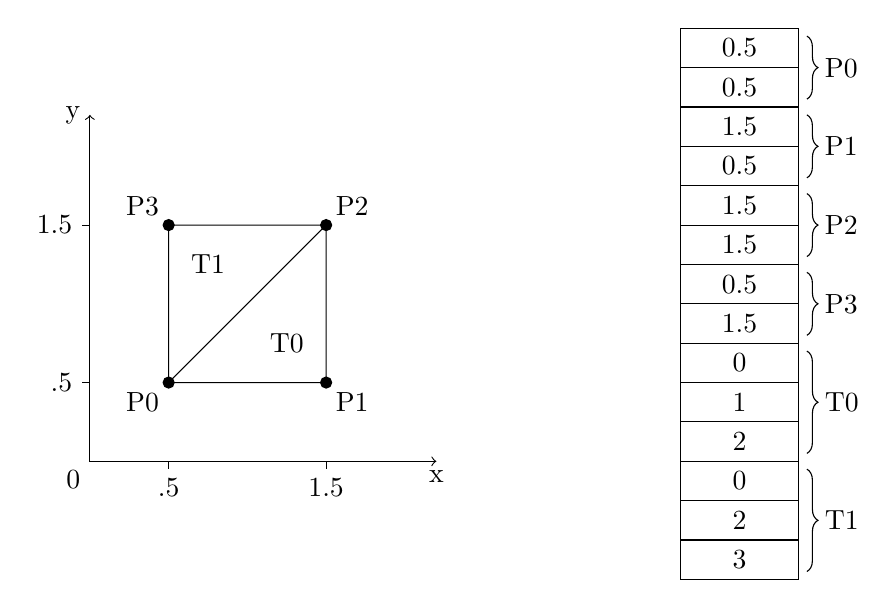
\begin{tikzpicture}
		% 2D scene
		\begin{scope}[shift={(0,0)}, scale=2]
			\draw[<->] (2.2,0) node[below]{x} -- (0,0) -- (0,2.2) node[left]{y};
			\draw (.5,0) -- (.5,-0.05) node[below]{.5};
			\draw (1.5,0) -- (1.5,-0.05) node[below]{1.5};
			\draw (0,.5) -- (-0.05,.5) node[left]{.5};
			\draw (0,1.5) -- (-0.05,1.5) node[left]{1.5};
			\begin{scope}[shift={(0.5,0.5)}]
				\draw (0,0) -- (0,1) -- (1,1) -- (0,0) -- (1,0) -- (1,1);
				\filldraw (0,0) circle (1pt) node[below left]{P0};
				\filldraw (1,0) circle (1pt) node[below right]{P1};
				\filldraw (1,1) circle (1pt) node[above right]{P2};
				\filldraw (0,1) circle (1pt) node[above left]{P3};
				\node at (.25, .75) {T1};
				\node at (.75, .25) {T0};
			\end{scope}
			\node[below left] at (0,0) {0};
		\end{scope}

		\begin{scope}[shift={(9,5.5)}, xscale=1.5, rotate=180]
			\draw (0,7) -- (0,0) -- (1,0) -- (1,7); 

			\draw (0,.5) -- (1,.5);
			\node at (.5, .25) {0.5};

			\draw (0,1) -- (1,1);
			\node at (.5, .75) {0.5};

			\draw (0,1.5) -- (1,1.5);
			\node at (.5, 1.25) {1.5};

			\draw (0,2) -- (1,2);
			\node at (.5, 1.75) {0.5};

			\draw (0,2.5) -- (1,2.5);
			\node at (.5, 2.25) {1.5};

			\draw (0,3) -- (1,3);
			\node at (.5, 2.75) {1.5};

			\draw (0,3.5) -- (1,3.5);
			\node at (.5, 3.25) {0.5};

			\draw (0,4) -- (1,4);
			\node at (.5, 3.75) {1.5};

			\draw (0,4.5) -- (1,4.5);
			\node at (.5, 4.25) {0};

			\draw (0,5) -- (1,5);
			\node at (.5, 4.75) {1};

			\draw (0,5.5) -- (1,5.5);
			\node at (.5, 5.25) {2};

			\draw (0,6) -- (1,6);
			\node at (.5, 5.75) {0};

			\draw (0,6.5) -- (1,6.5);
			\node at (.5, 6.25) {2};

			\draw (0,7) -- (1,7);
			\node at (.5, 6.75) {3};

			\draw [decorate,decoration={brace,amplitude=4pt},xshift=-2pt]
			(0,0.1) -- (0,0.9) node [right,midway,xshift=3pt]{P0};
			\draw [decorate,decoration={brace,amplitude=4pt},xshift=-2pt]
			(0,1.1) -- (0,1.9) node [right,midway,xshift=3pt]{P1};
			\draw [decorate,decoration={brace,amplitude=4pt},xshift=-2pt]
			(0,2.1) -- (0,2.9) node [right,midway,xshift=3pt]{P2};
			\draw [decorate,decoration={brace,amplitude=4pt},xshift=-2pt]
			(0,3.1) -- (0,3.9) node [right,midway,xshift=3pt]{P3};

			\draw [decorate,decoration={brace,amplitude=4pt},xshift=-2pt]
			(0,4.1) -- (0,5.4) node [right,midway,xshift=3pt]{T0};
			\draw [decorate,decoration={brace,amplitude=4pt},xshift=-2pt]
			(0,5.6) -- (0,6.9) node [right,midway,xshift=3pt]{T1};
		\end{scope}
	\end{tikzpicture}

	\caption{Geometry example. To simplify, a 2-dimensional case is presented. On the right a simple triangulated mesh is shown, on the left there is a valid binary file. A corresponding JSON file is shown in Listing \ref{scene_json}.}
	\label{scene_bin}
\end{figure}

\begin{Listing}
	\begin{lstlisting}
{
	"camera": {...},
	"render": {...},
	"geometries": [
		{
			"name":     "quad",
			"material": {...},
			"buffers": [
				{
					"offset": 0,
					"size":   32,
					"type":   "vertices"
				},
				{
				 	"offset": 32,
				 	"size":   24,
				 	"type":   "indices"
				}
			]
		}
	]
}
	\end{lstlisting}
	\caption{JSON scene file example relative to Figure \ref{scene_bin}. Information not relative to the geometry shape has been omitted. Please also remember this is a 2-dimensional example, hence the vertex buffer size is only 2 dimensions * 4 points * 4 bytes = 32 bytes instead of being 48 bytes like it would be in the ordinary 3-dimensional case.}
	\label{scene_json}
\end{Listing}